\subsection*{Appendix B: DRE19 Examples}\label{appendix: B}
Presented below, in \autoref{fig:appb1}, representative examples of the 6 different classes in the DRE19 dataset.

\begin{figure}[H]
  \centering % <-- added
  \begin{subfigure}{0.3\textwidth}
    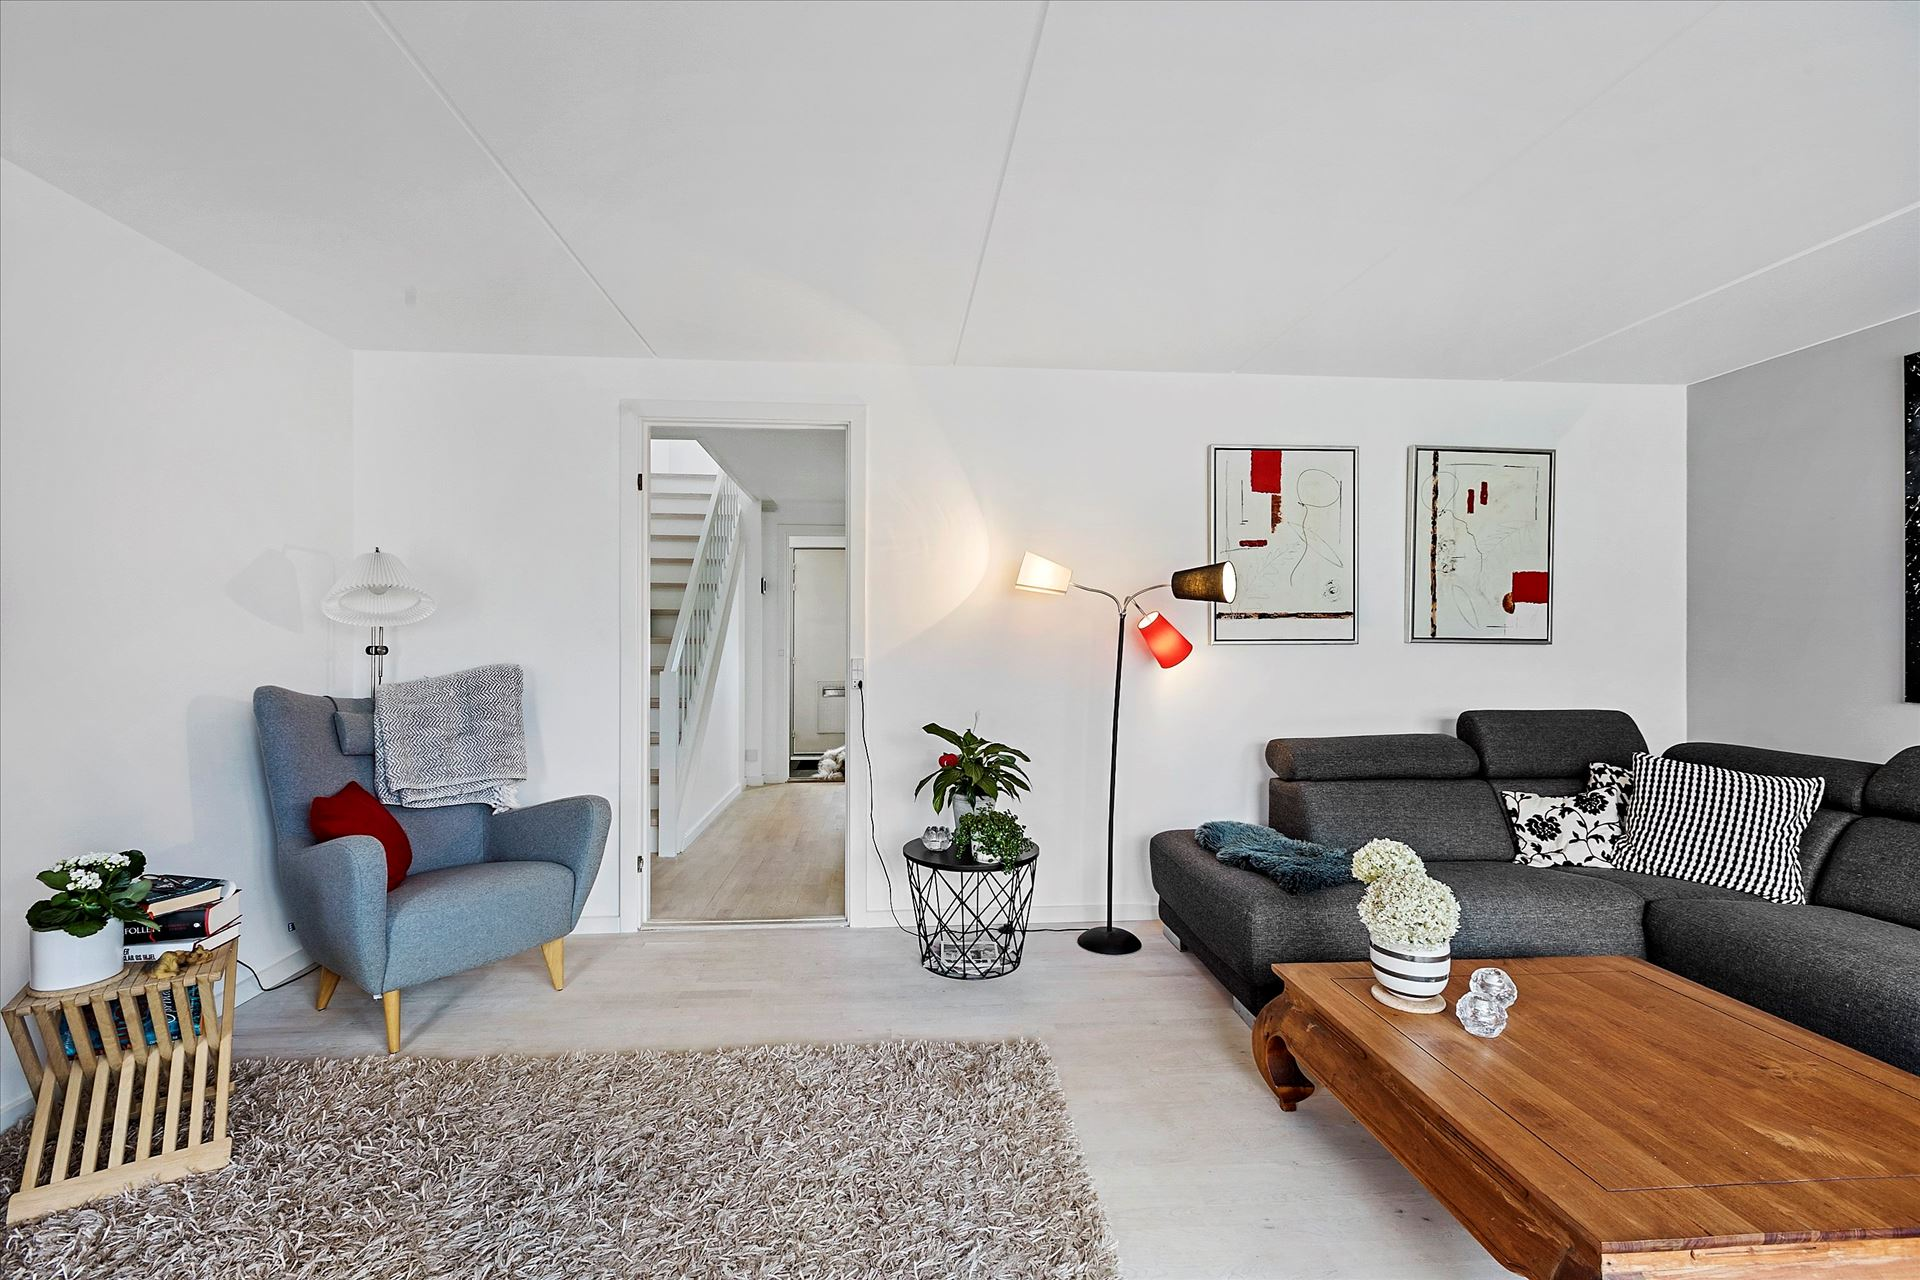
\includegraphics[width=\linewidth]{pictures/random/example_livingroom}
    \caption{Living Room}
  \end{subfigure}\hfil % <-- added
  \begin{subfigure}{0.3\textwidth}
    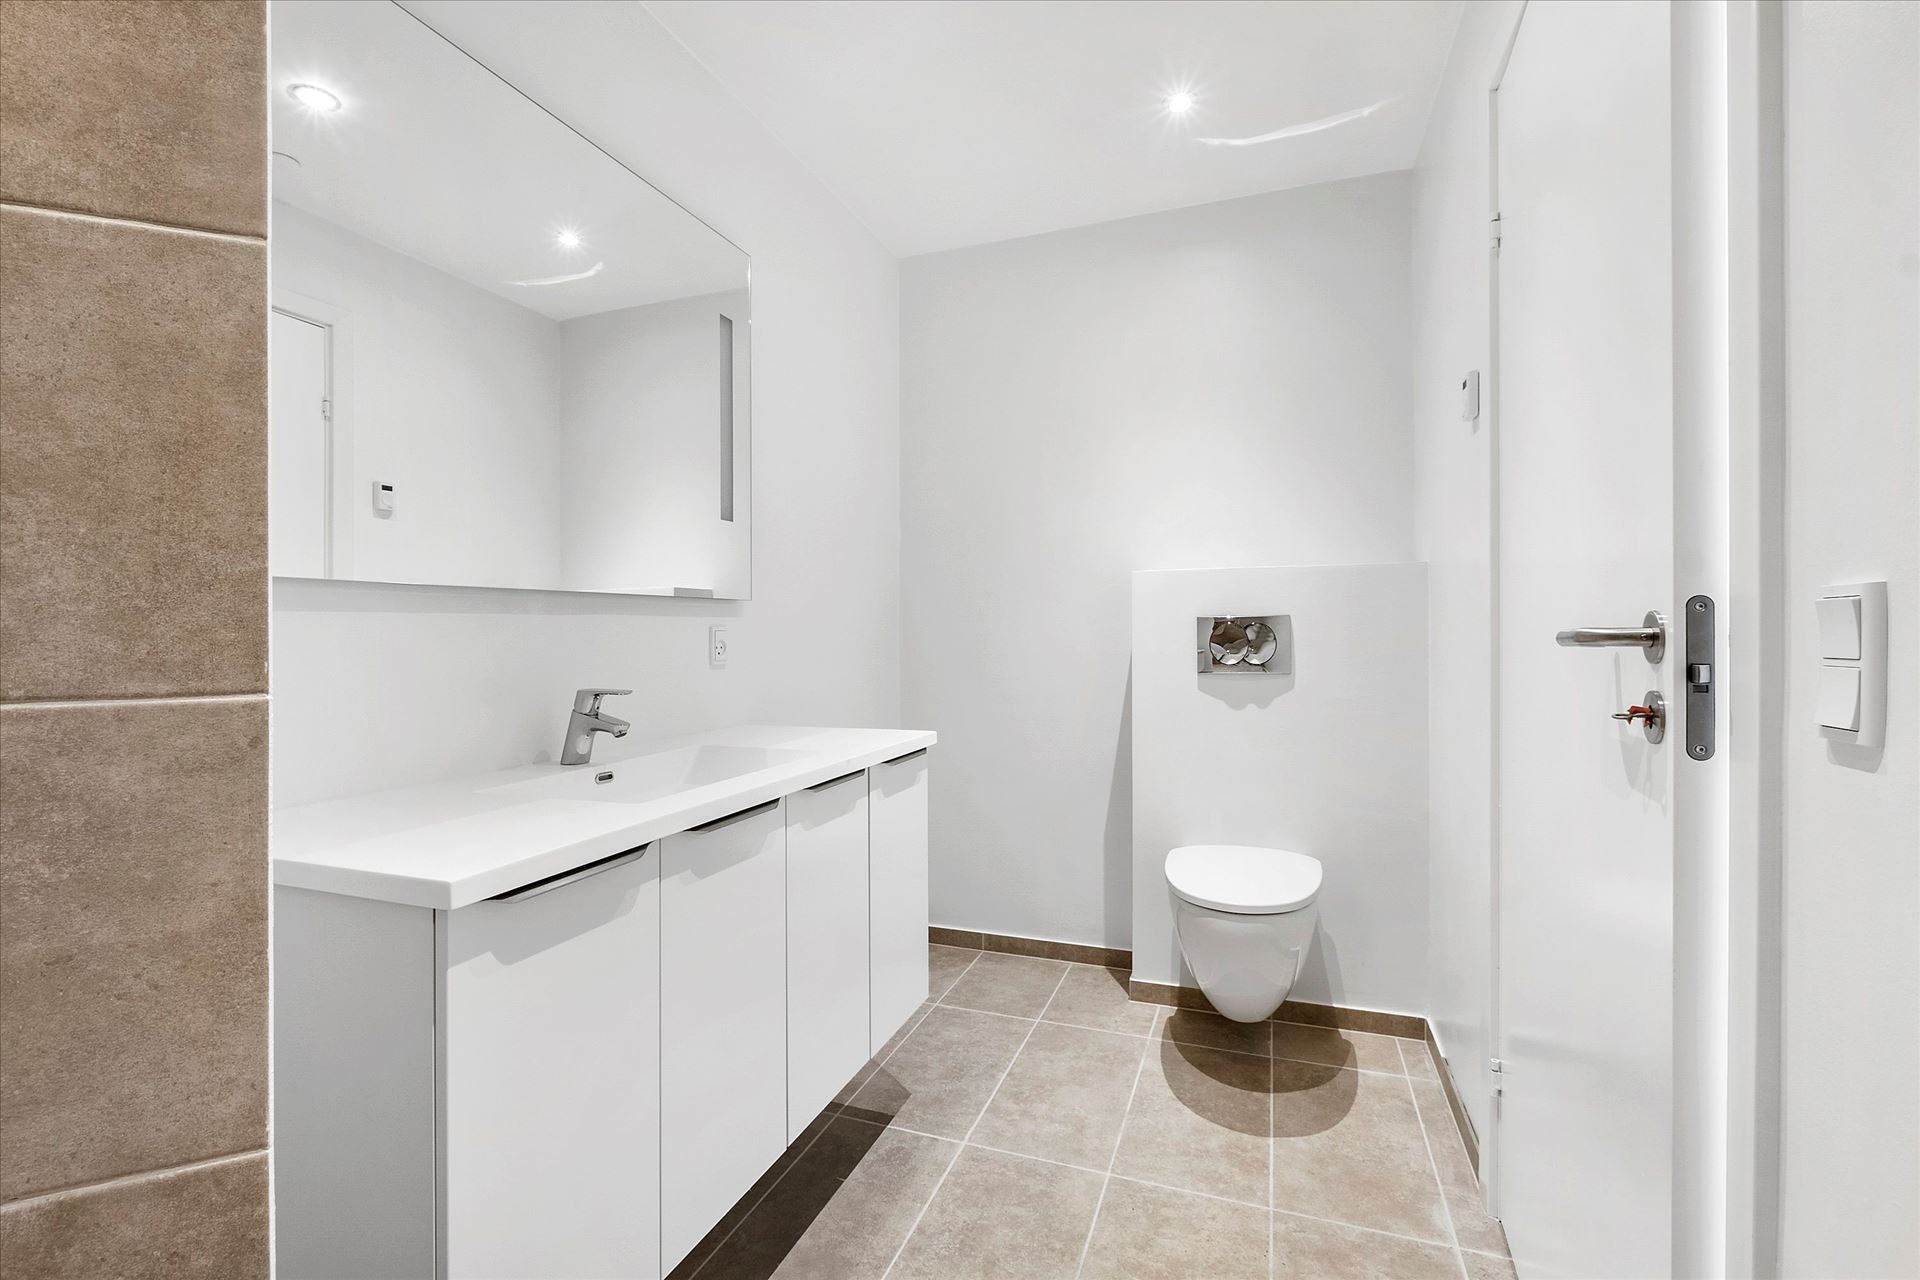
\includegraphics[width=\linewidth]{pictures/random/example_bathroom}
    \caption{Bathroom}
  \end{subfigure}\hfil % <-- added
  \begin{subfigure}{0.3\textwidth}
    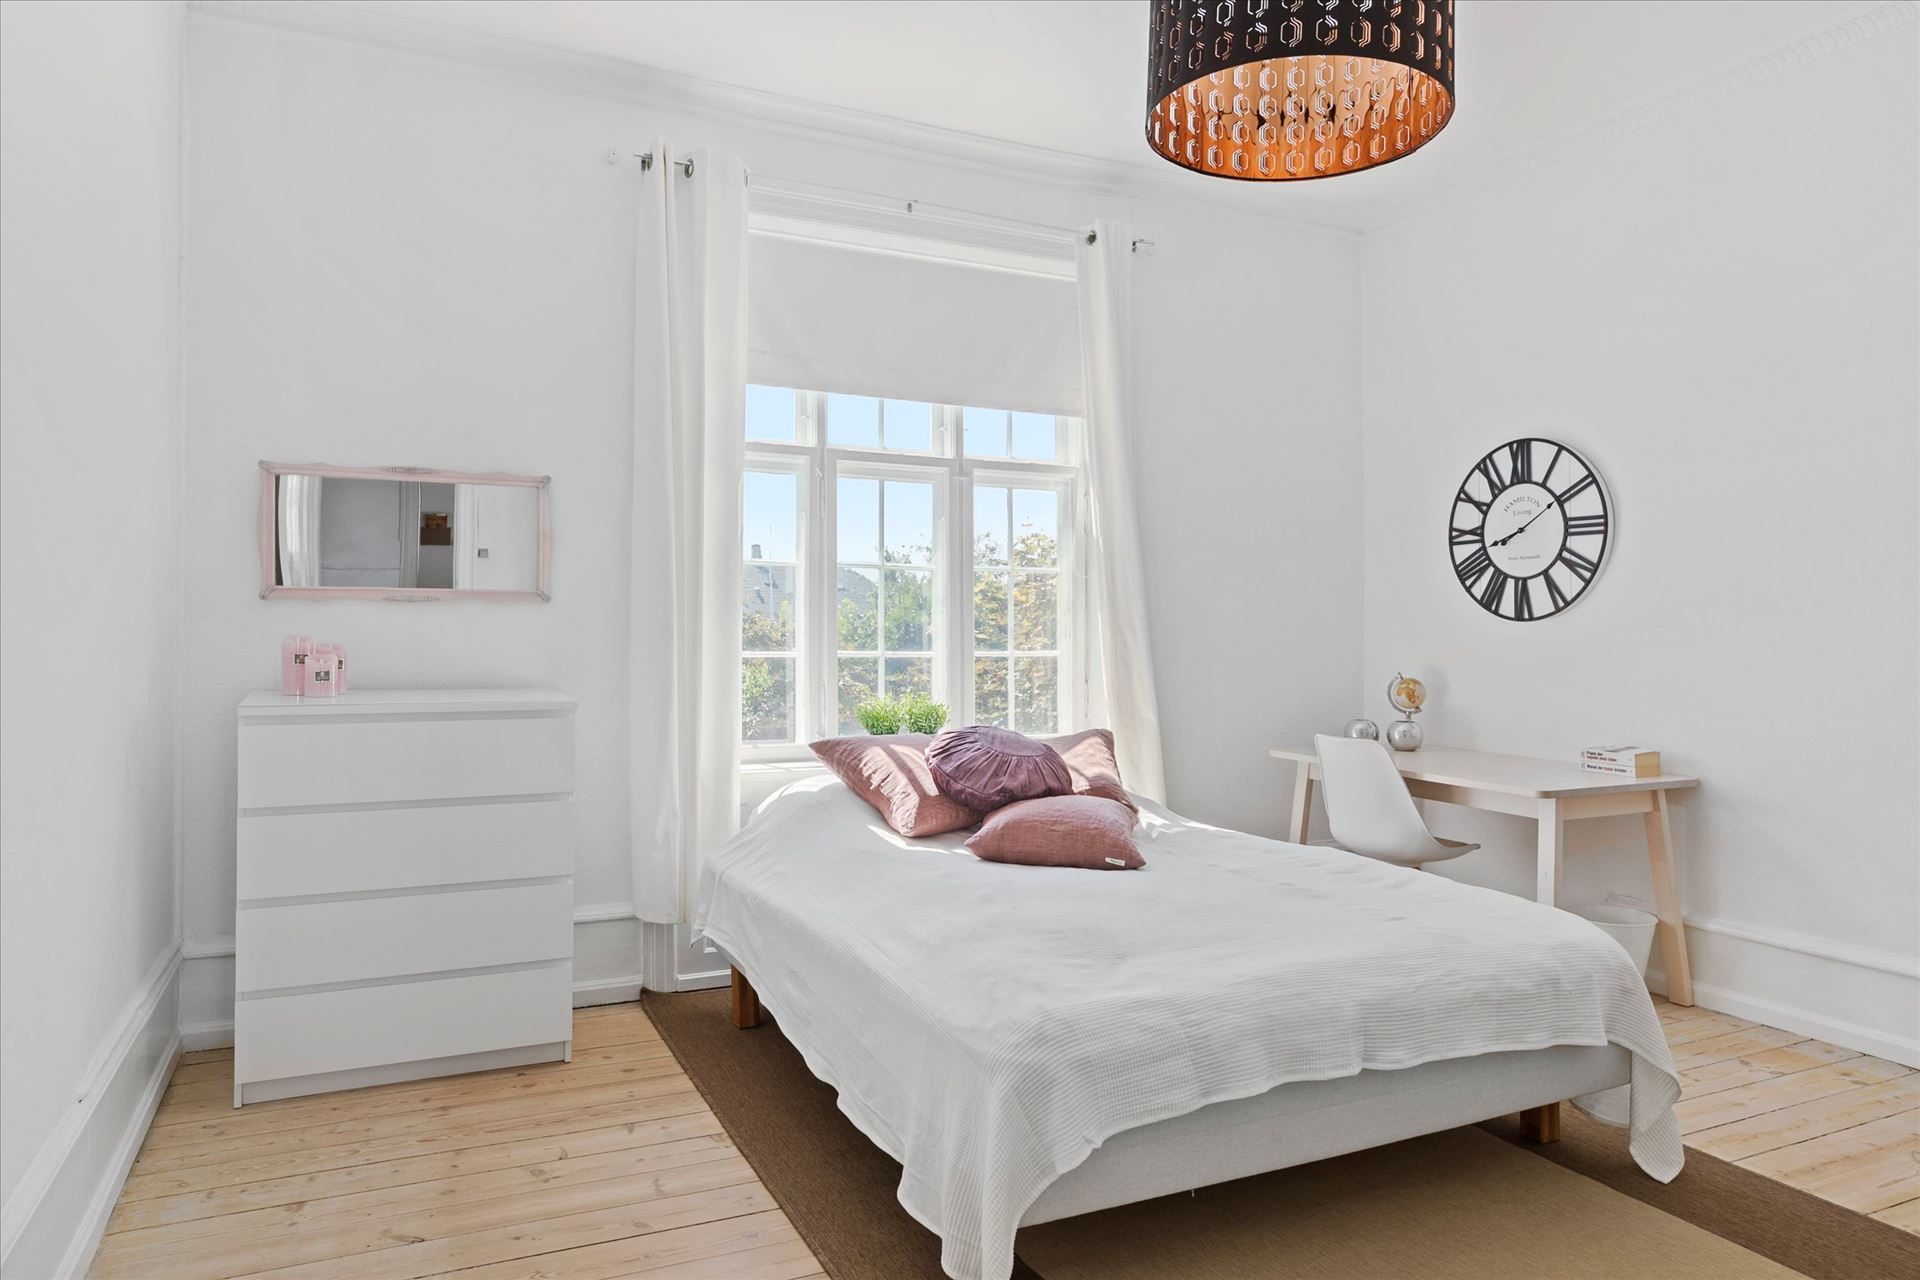
\includegraphics[width=\linewidth]{pictures/random/example_bedroom}
    \caption{Bedroom}
  \end{subfigure}
  \medskip
  \begin{subfigure}{0.3\textwidth}
    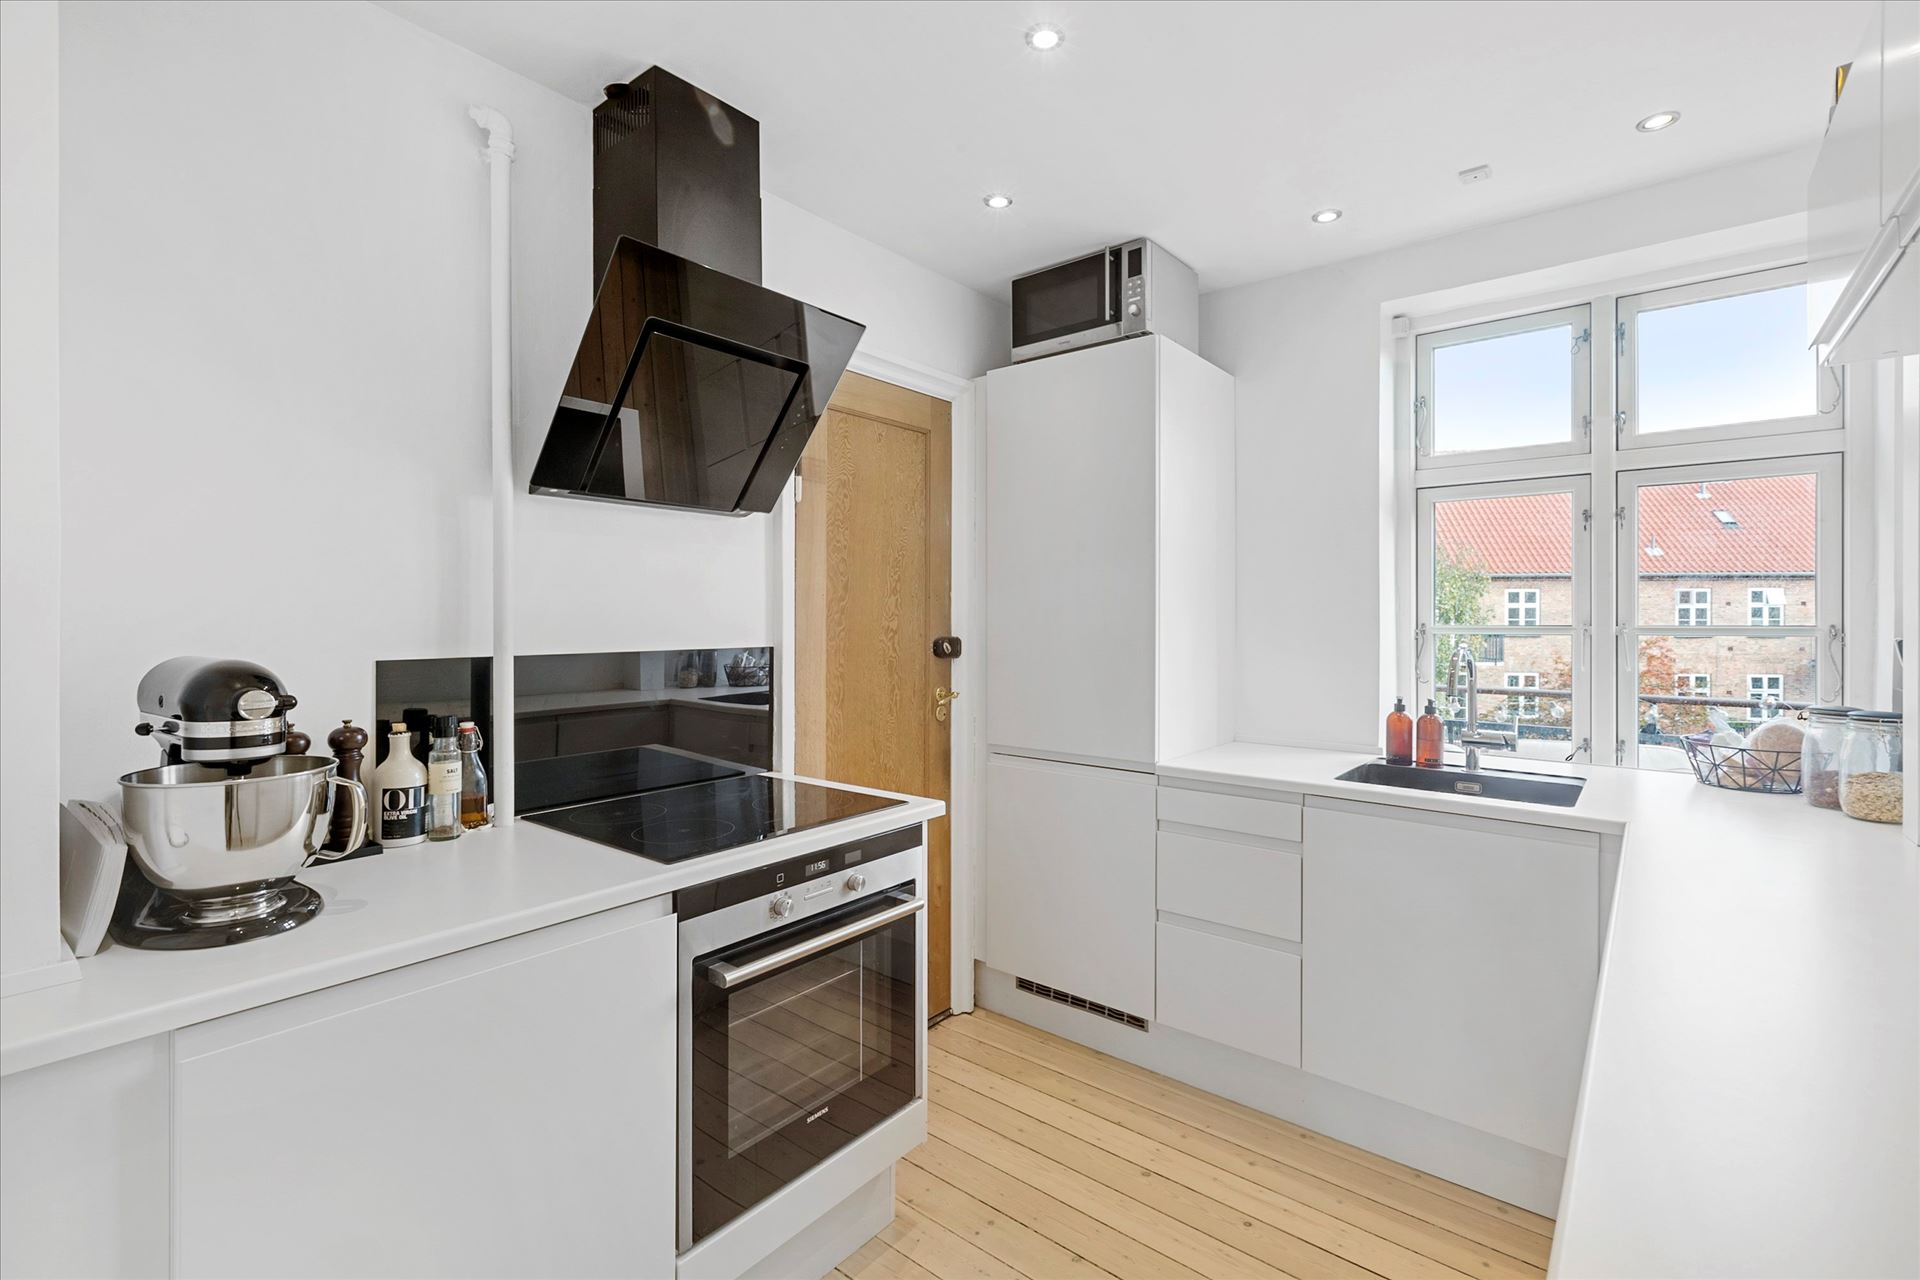
\includegraphics[width=\linewidth]{pictures/random/example_kitchen}
    \caption{Kitchen}
  \end{subfigure}\hfil % <-- added
  \begin{subfigure}{0.3\textwidth}
    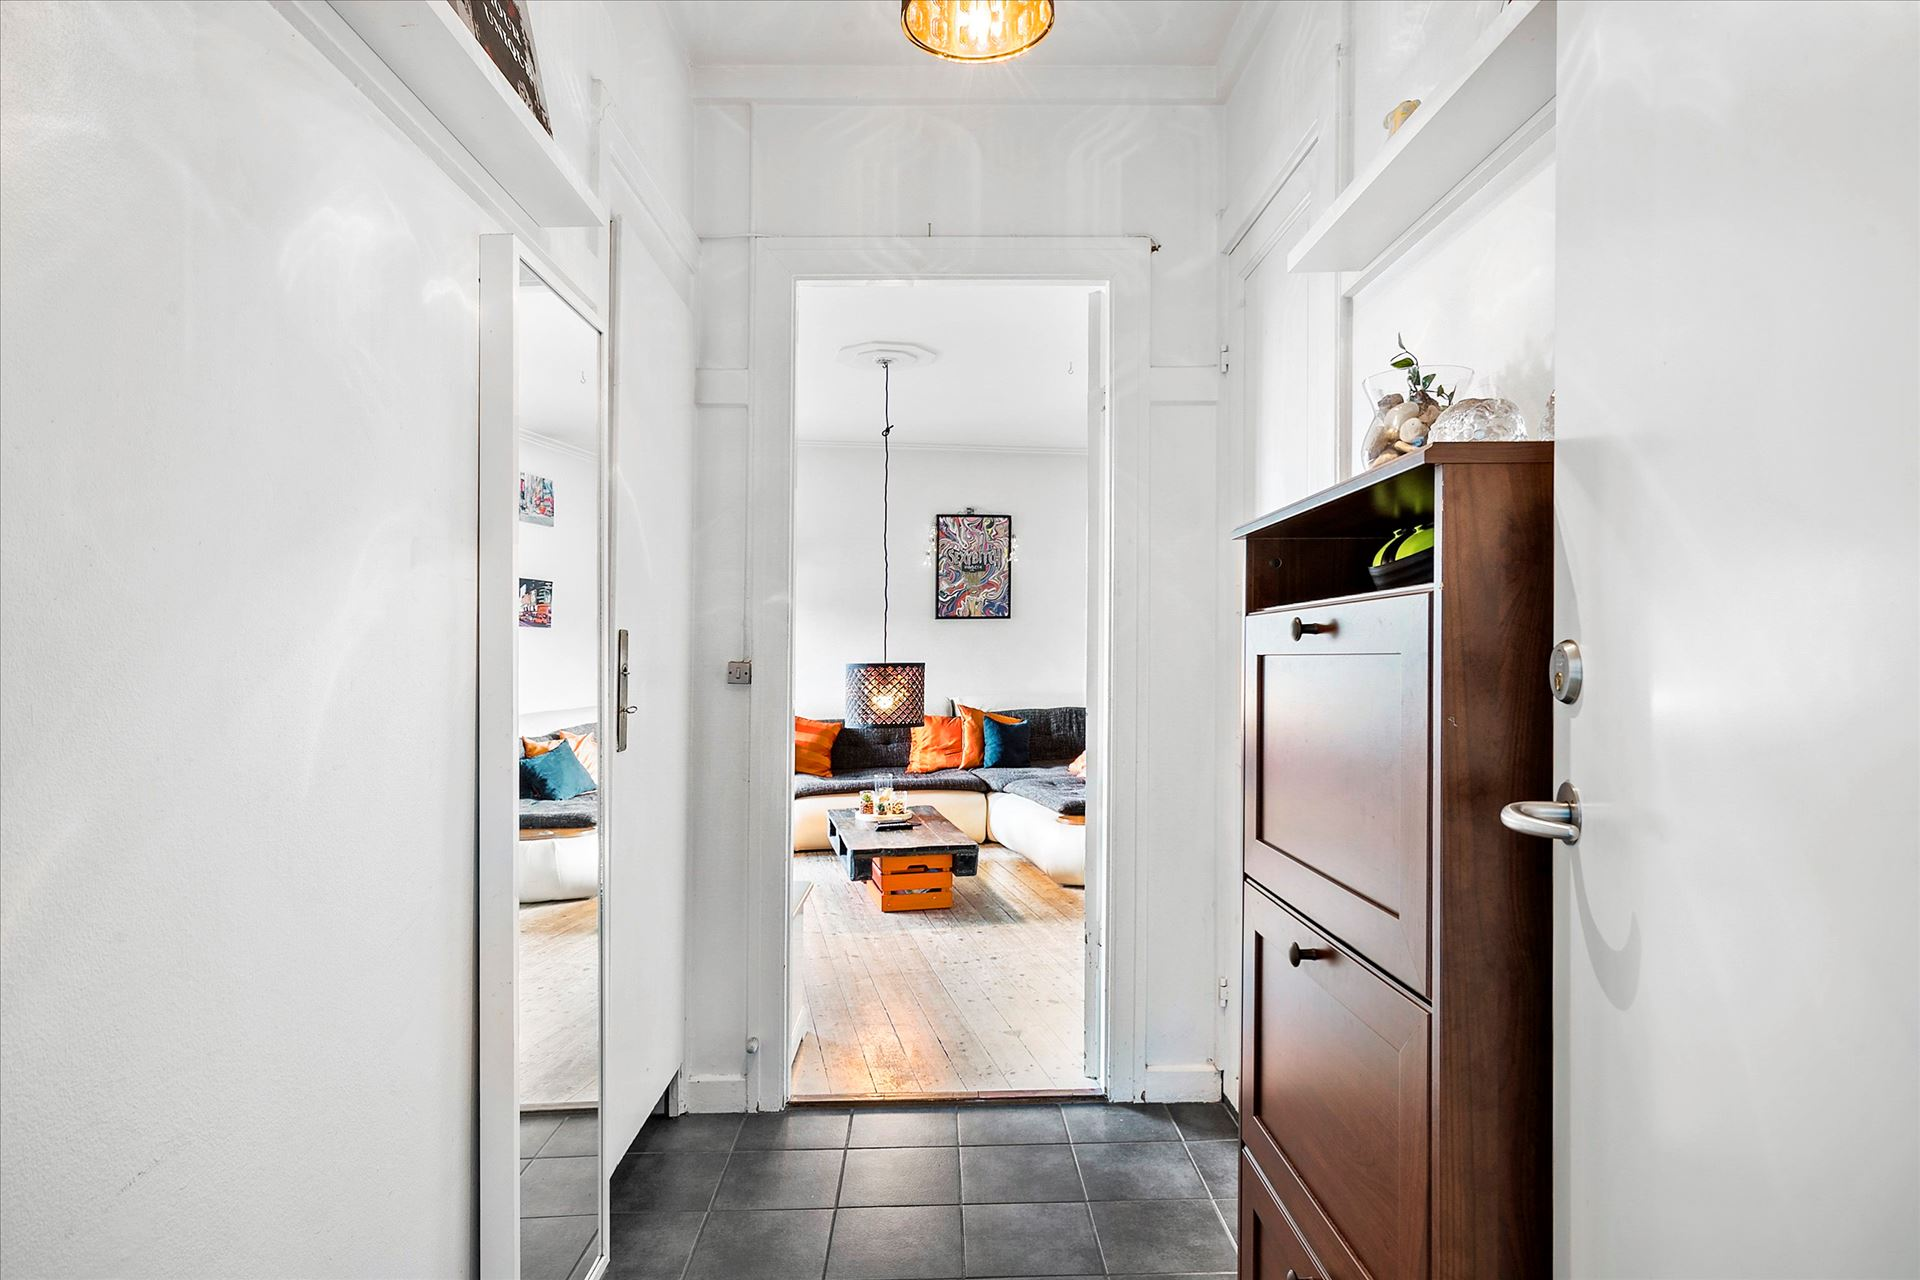
\includegraphics[width=\linewidth]{pictures/random/example_entre}
    \caption{Entre}
  \end{subfigure}\hfil % <-- added
  \begin{subfigure}{0.3\textwidth}
    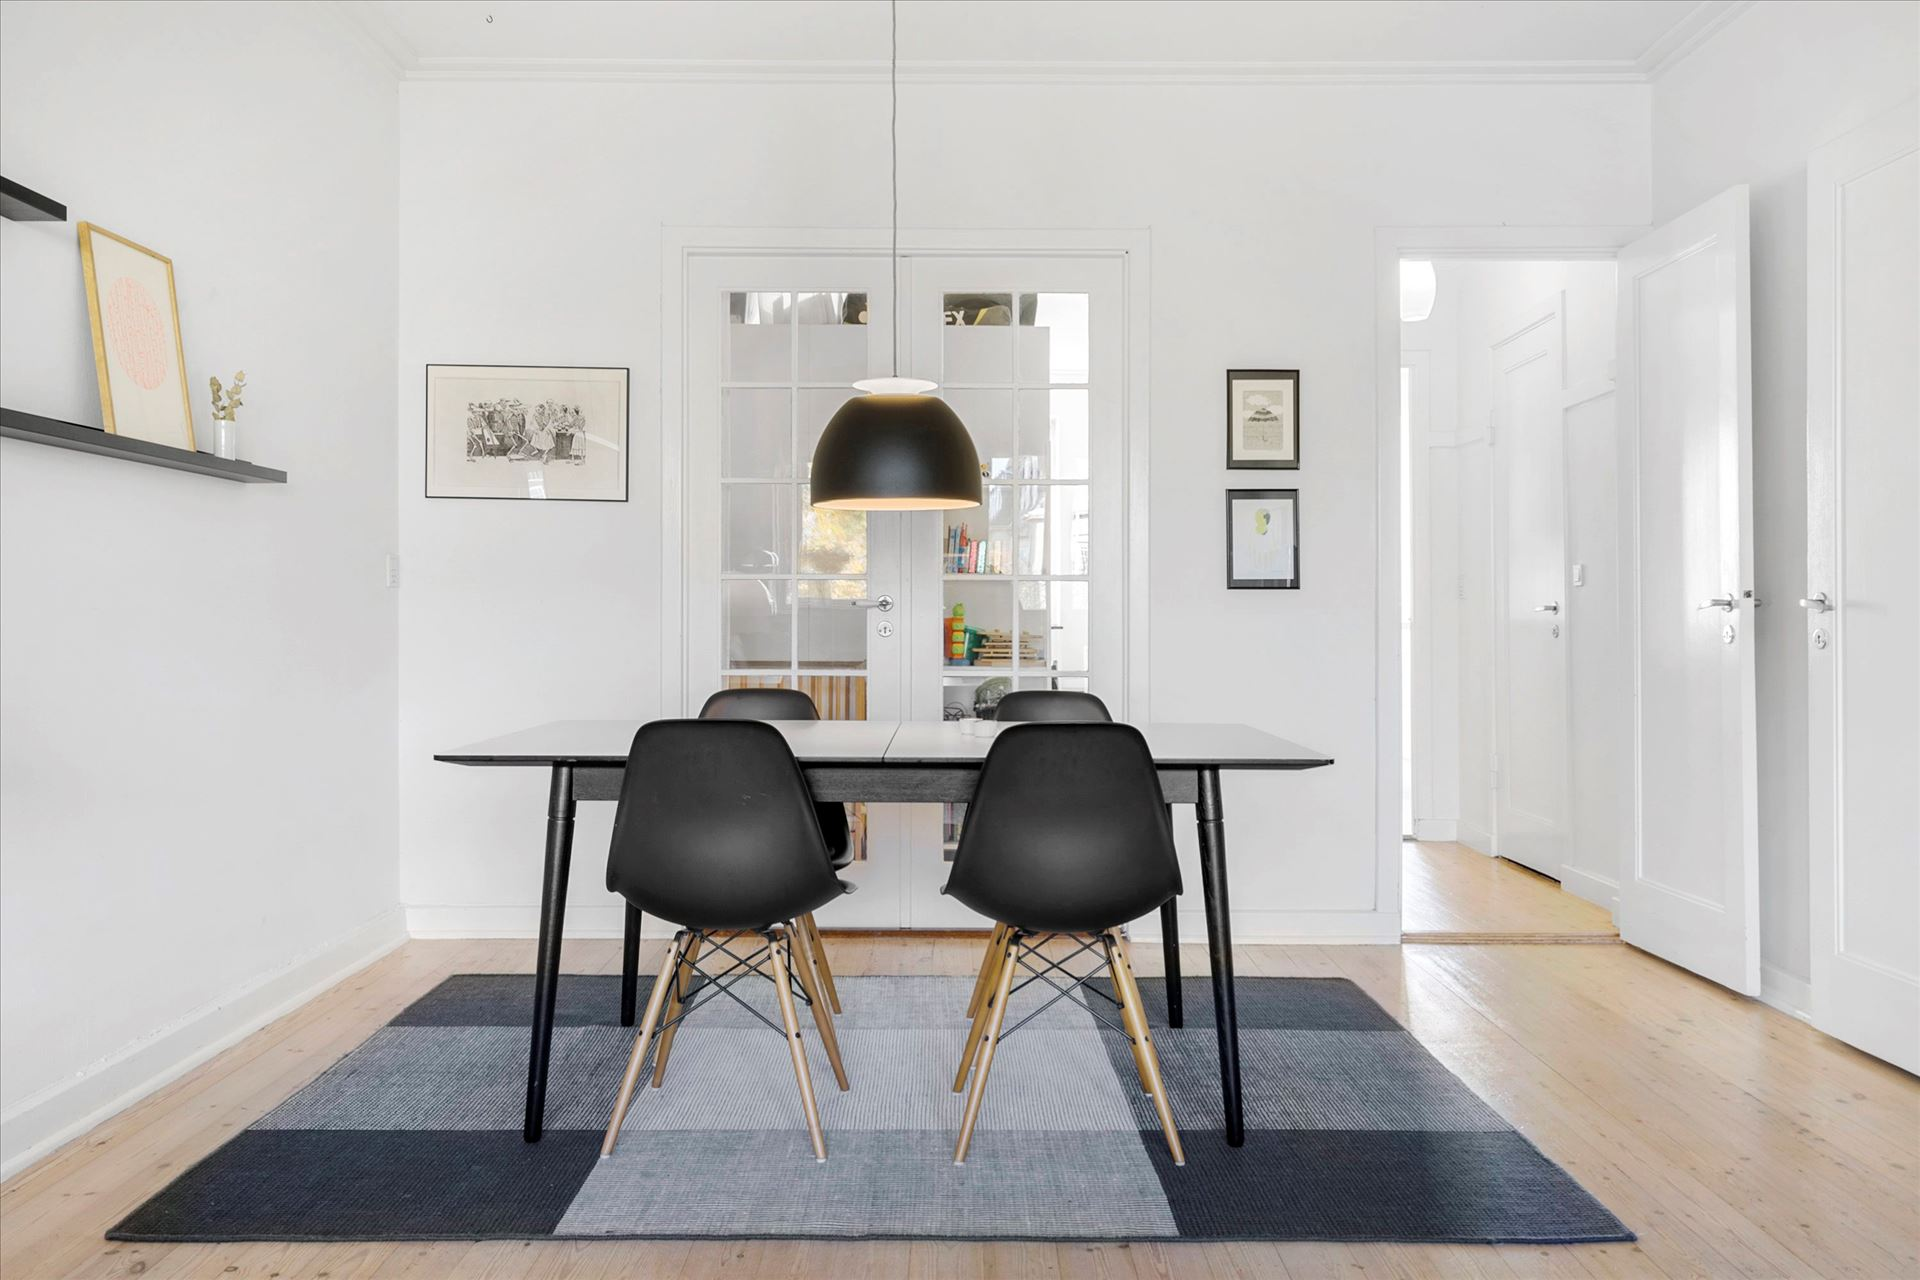
\includegraphics[width=\linewidth]{pictures/random/example_diningroom}
    \caption{Dining Room}
  \end{subfigure}
  \caption{Room Archetypes}
  \label{fig:appb1}
\end{figure}

Less representative images have also been added to every class. For these images it holds, that labeling by hand was not as straightforward as in the examples above. 
This can often be attributed to the photo angle being odd or that the image contents spans multiple room classes. 
It has been the authors labeling strategy to try and infer the room type based on the images most prevalent features.

\begin{figure}[H]
  \centering % <-- added
  \begin{subfigure}{0.3\textwidth}
    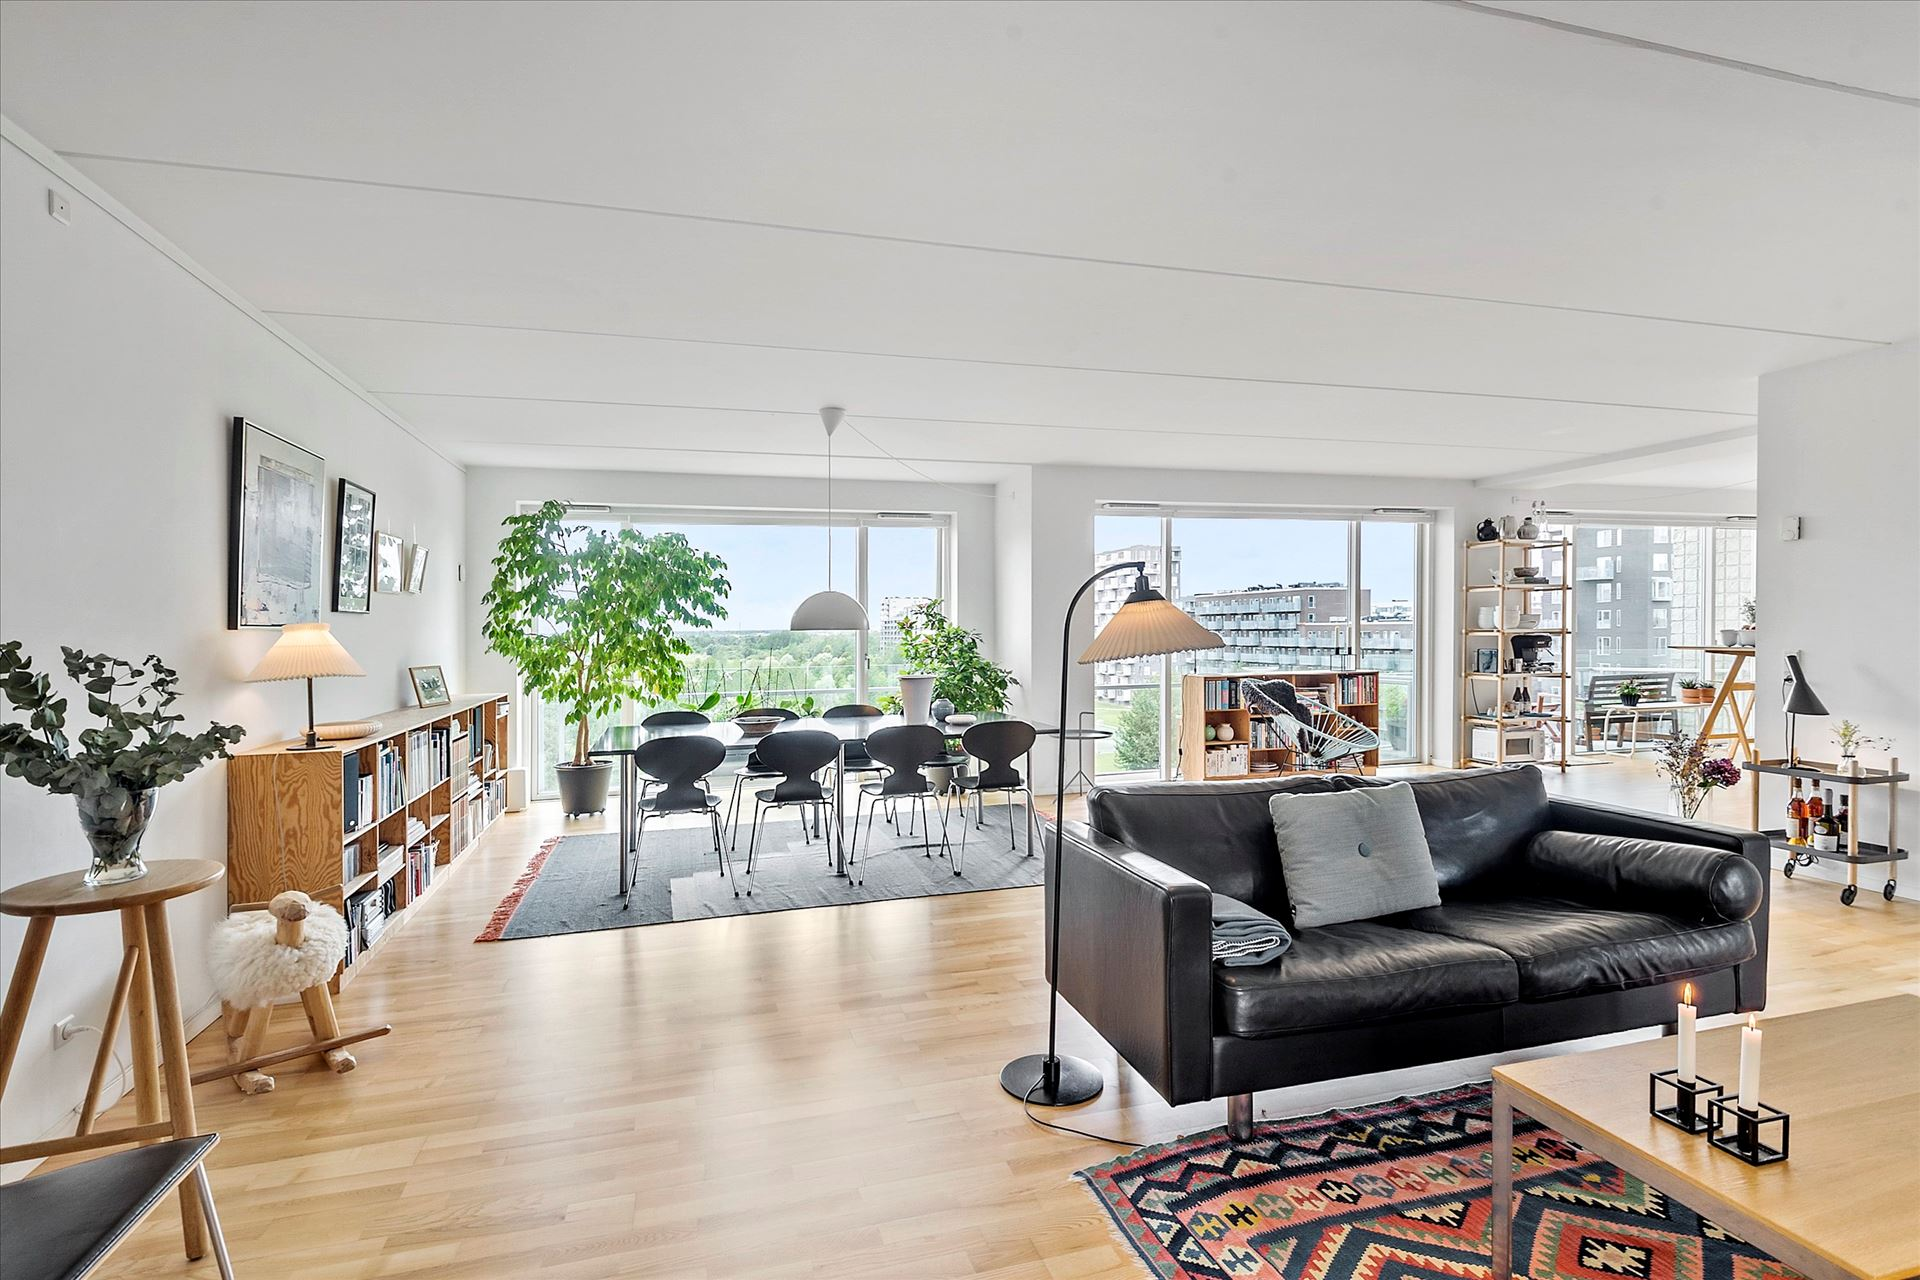
\includegraphics[width=\linewidth]{pictures/random/bexample_livingroom}
    \caption{Living Room}
  \end{subfigure}\hfil % <-- added
  \begin{subfigure}{0.3\textwidth}
    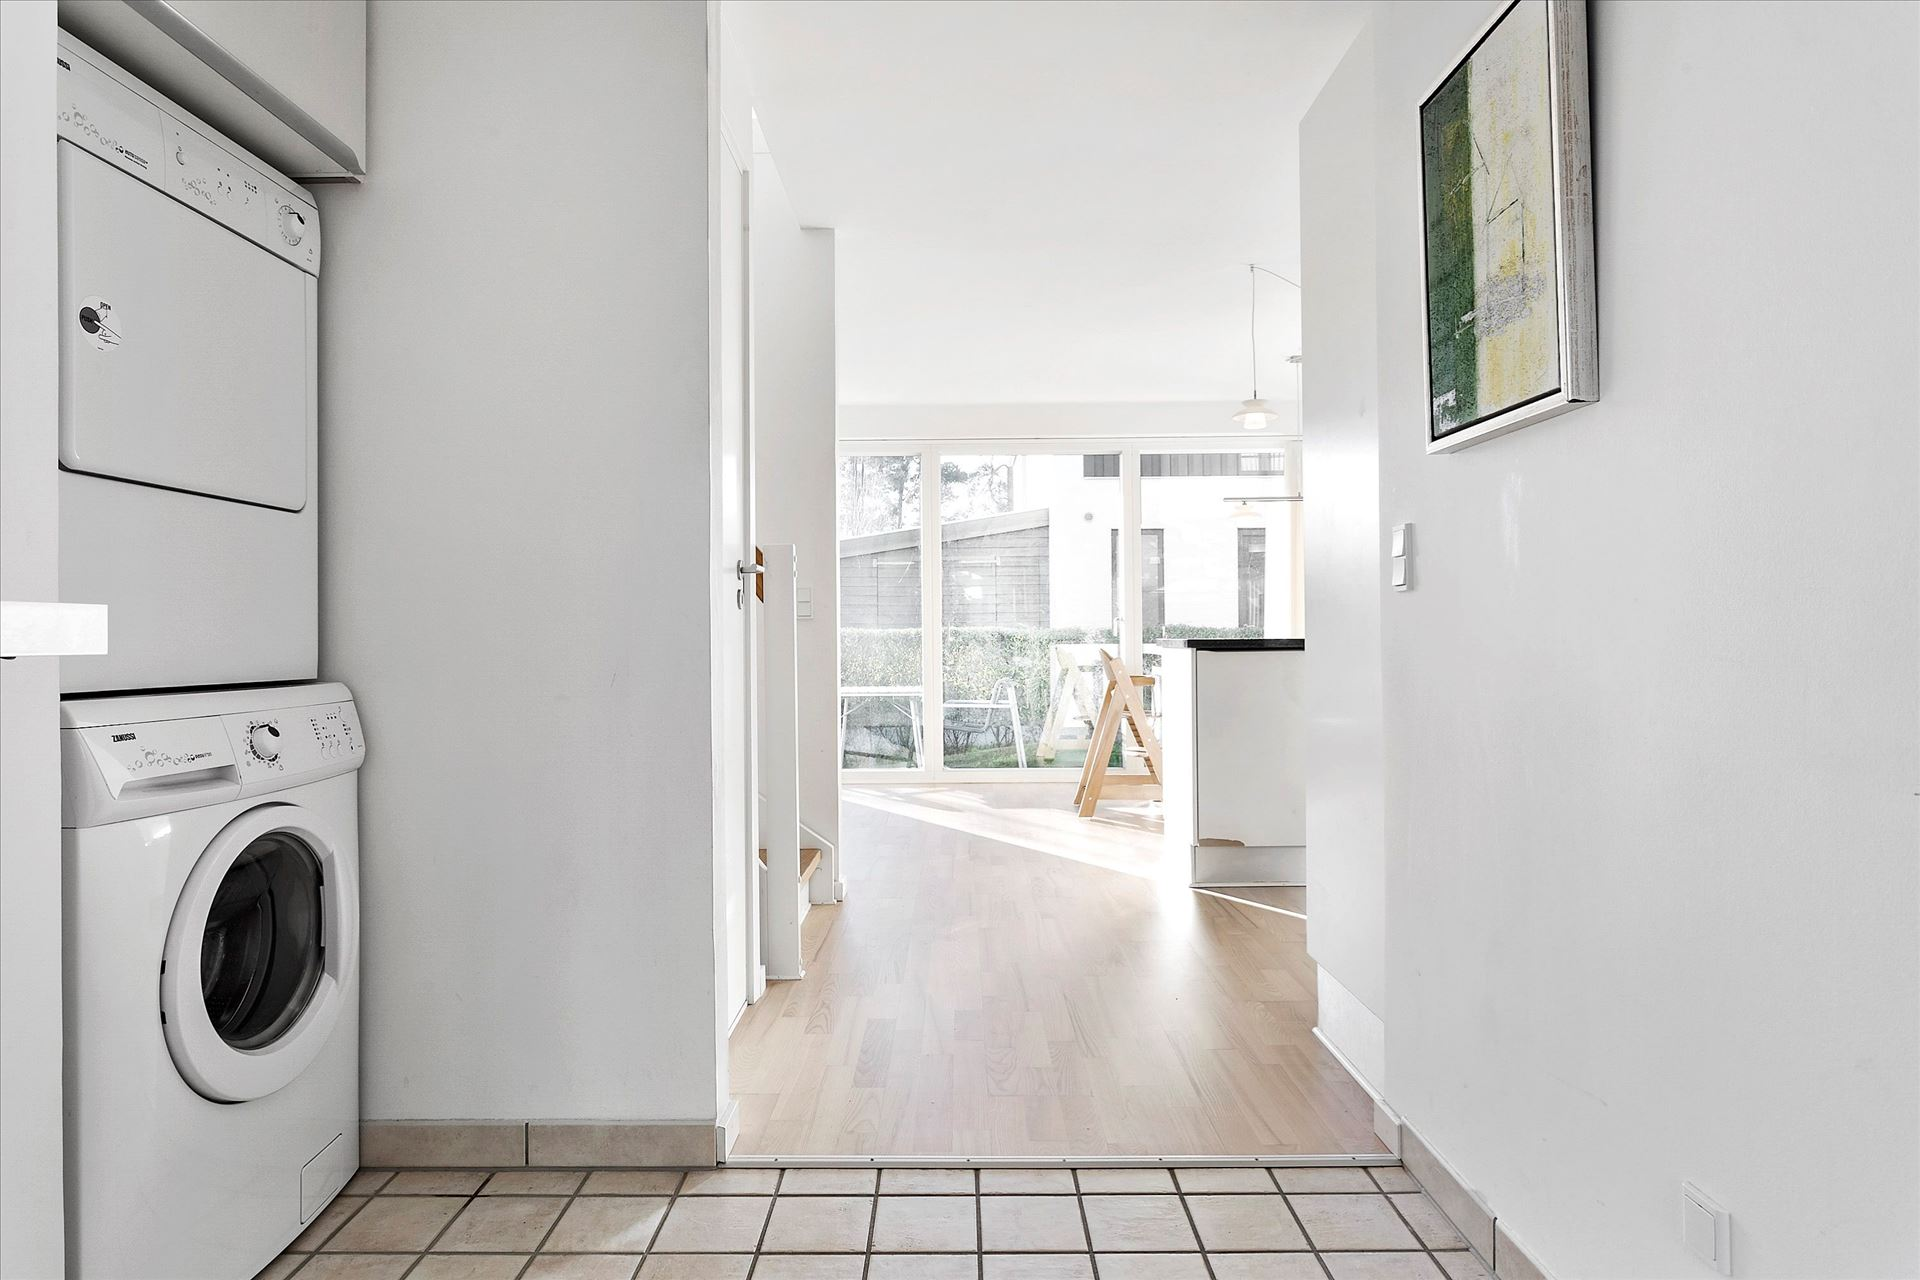
\includegraphics[width=\linewidth]{pictures/random/bexample_bathroom}
    \caption{Bathroom}
  \end{subfigure}\hfil % <-- added
  \begin{subfigure}{0.3\textwidth}
    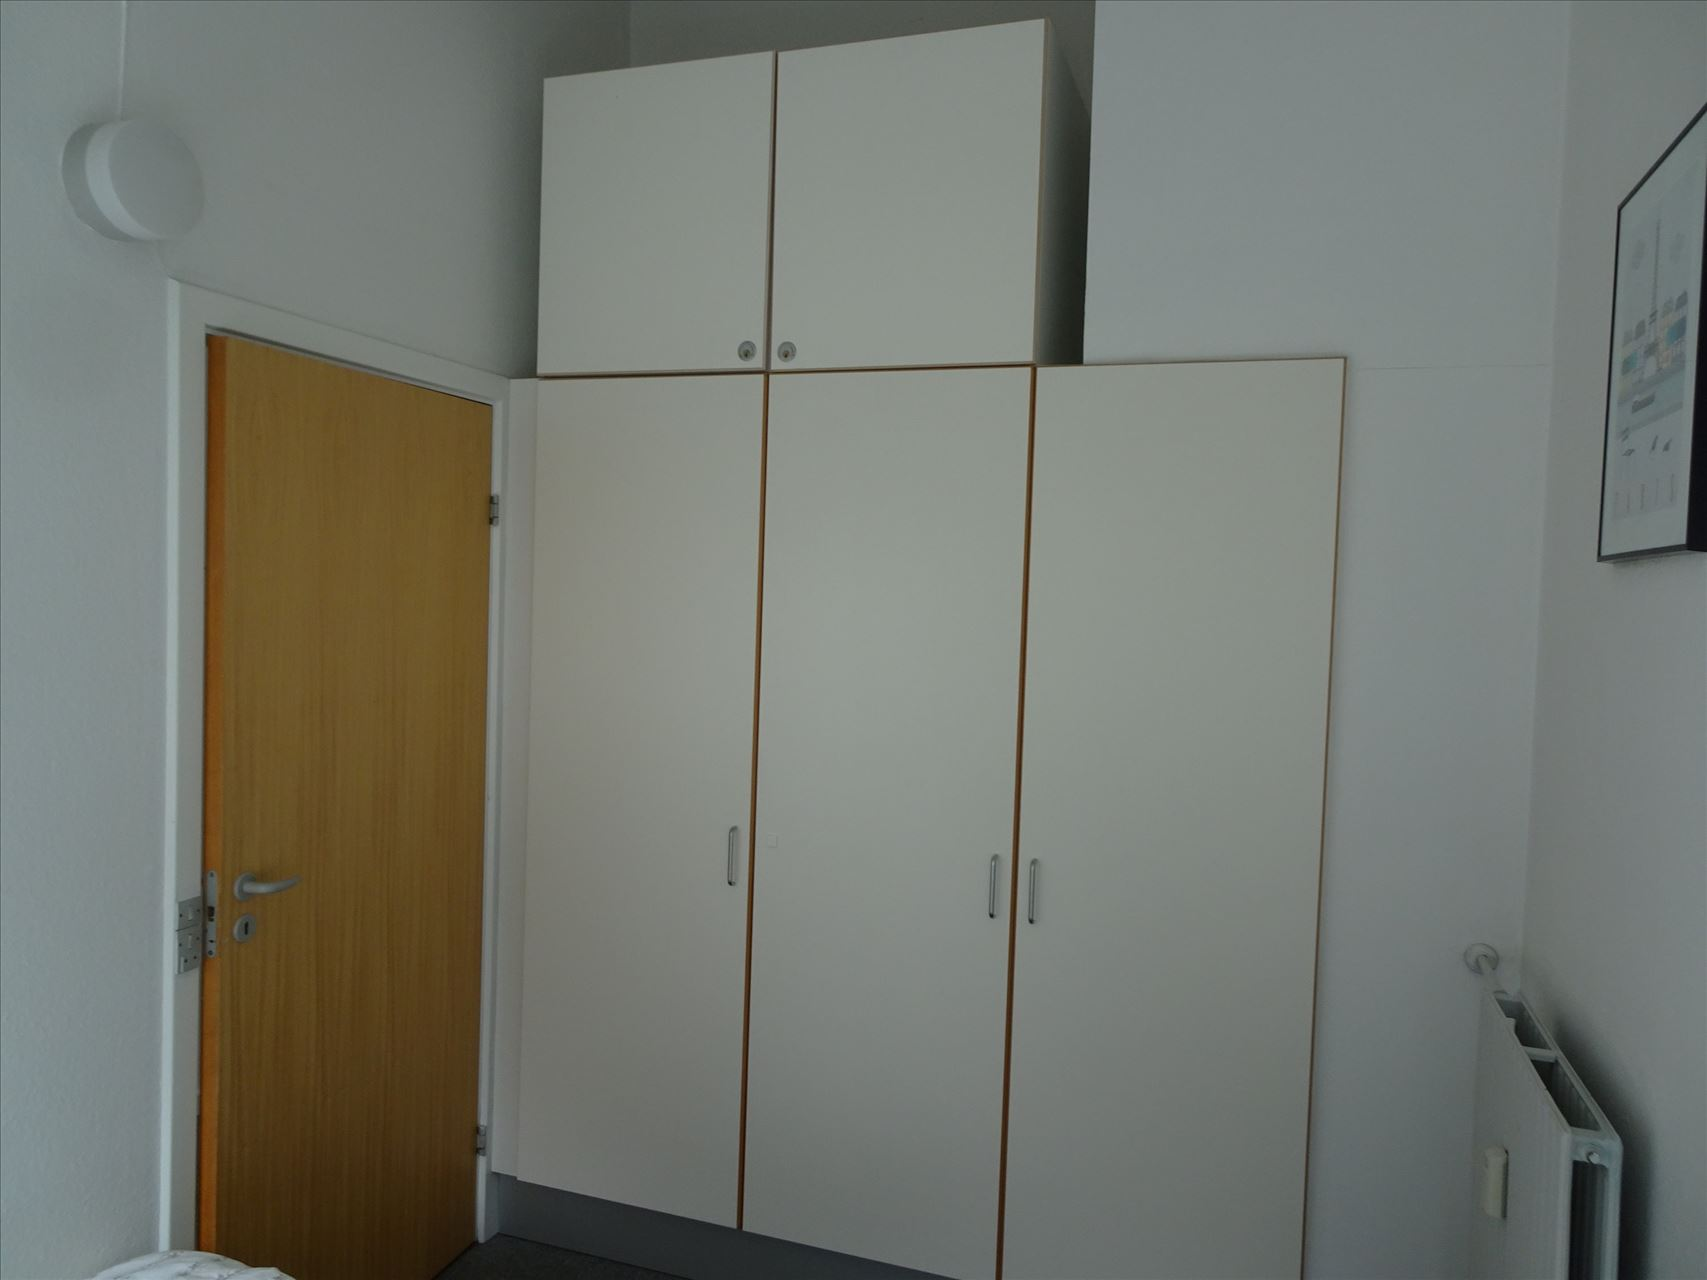
\includegraphics[width=\linewidth]{pictures/random/bexample_bedroom}
    \caption{Bedroom}
  \end{subfigure}
  \medskip
  \begin{subfigure}{0.3\textwidth}
    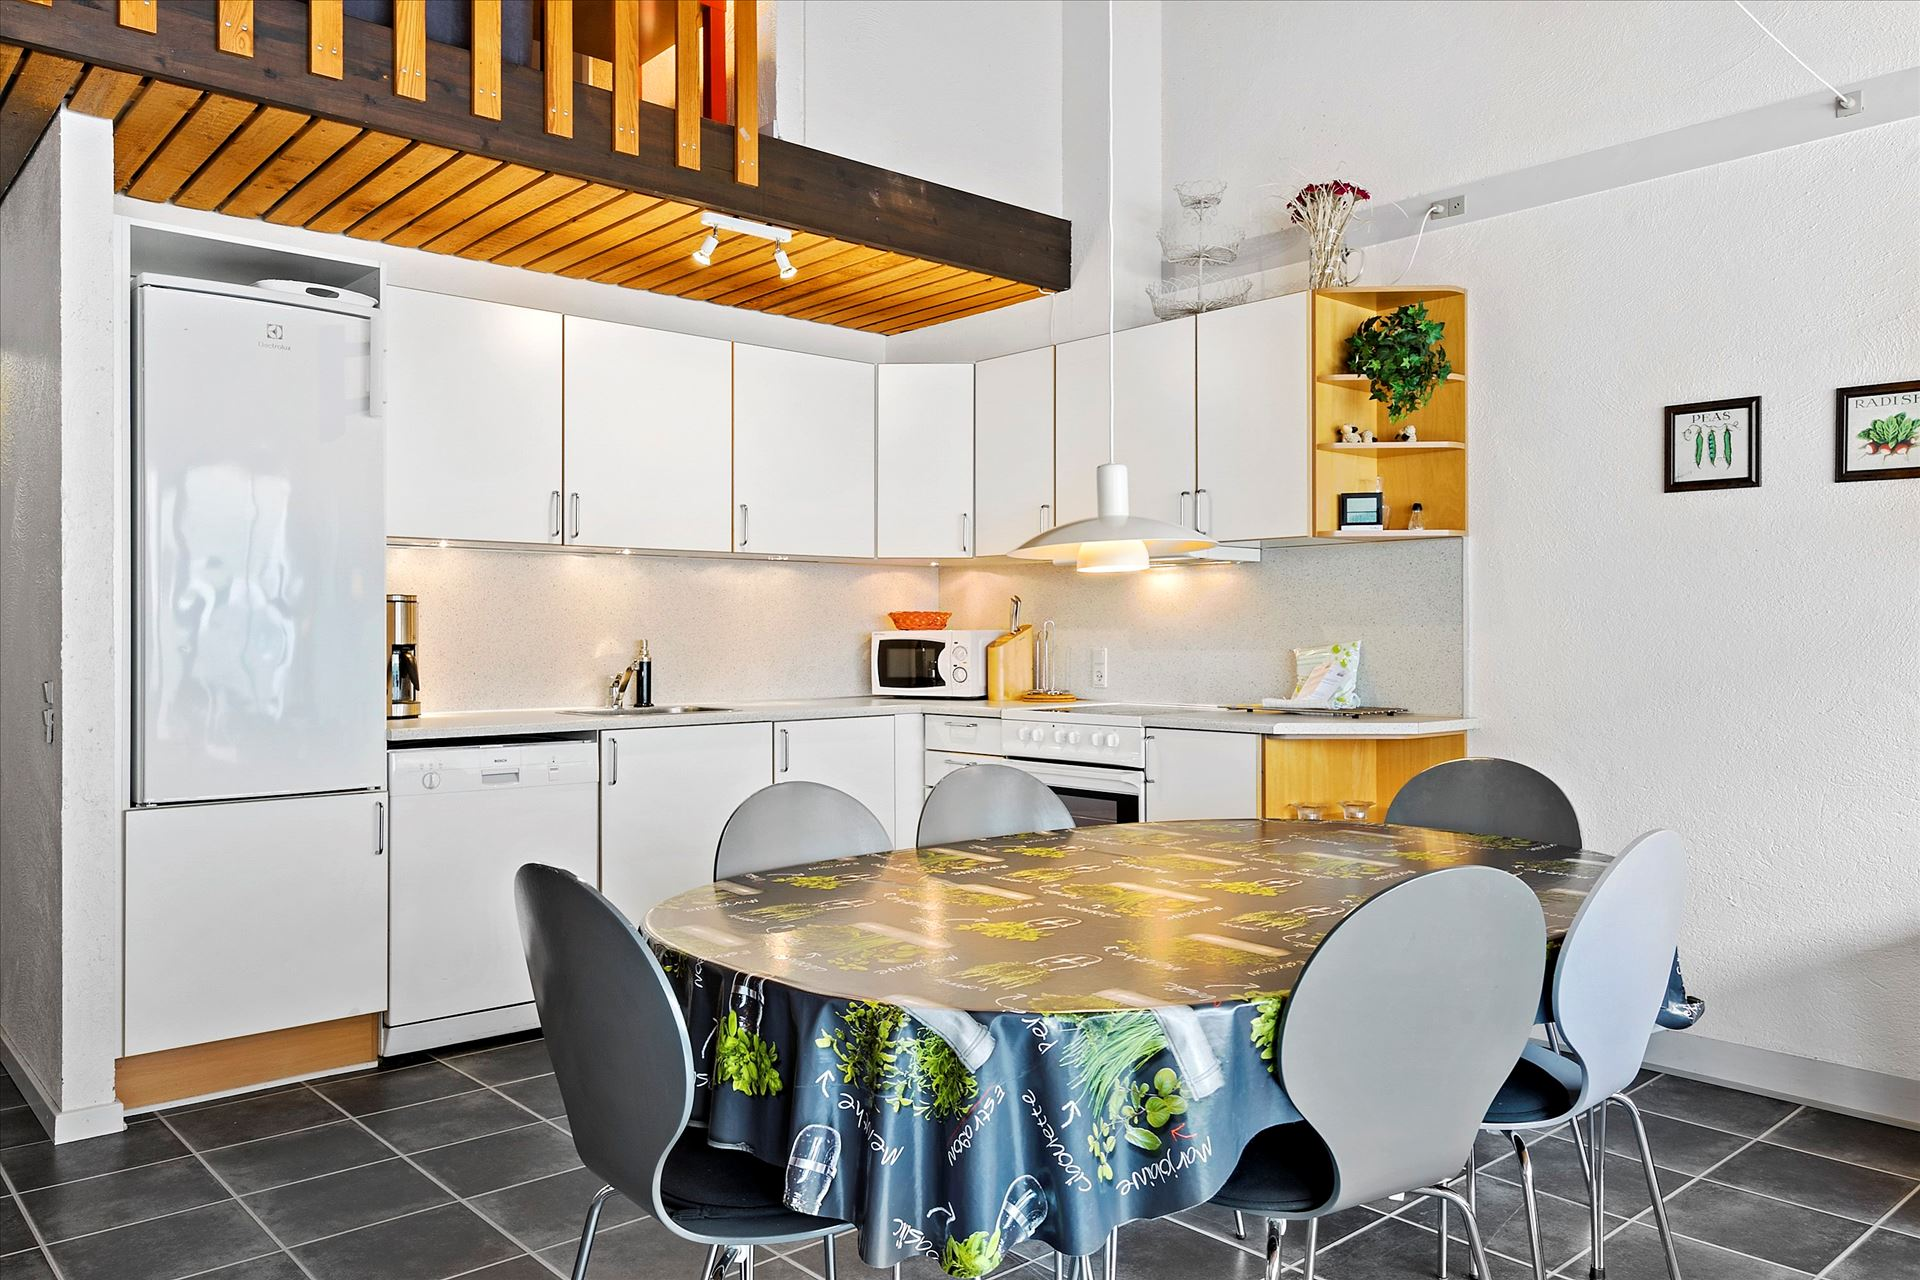
\includegraphics[width=\linewidth]{pictures/random/bexample_kitchen}
    \caption{Kitchen}
  \end{subfigure}\hfil % <-- added
  \begin{subfigure}{0.3\textwidth}
    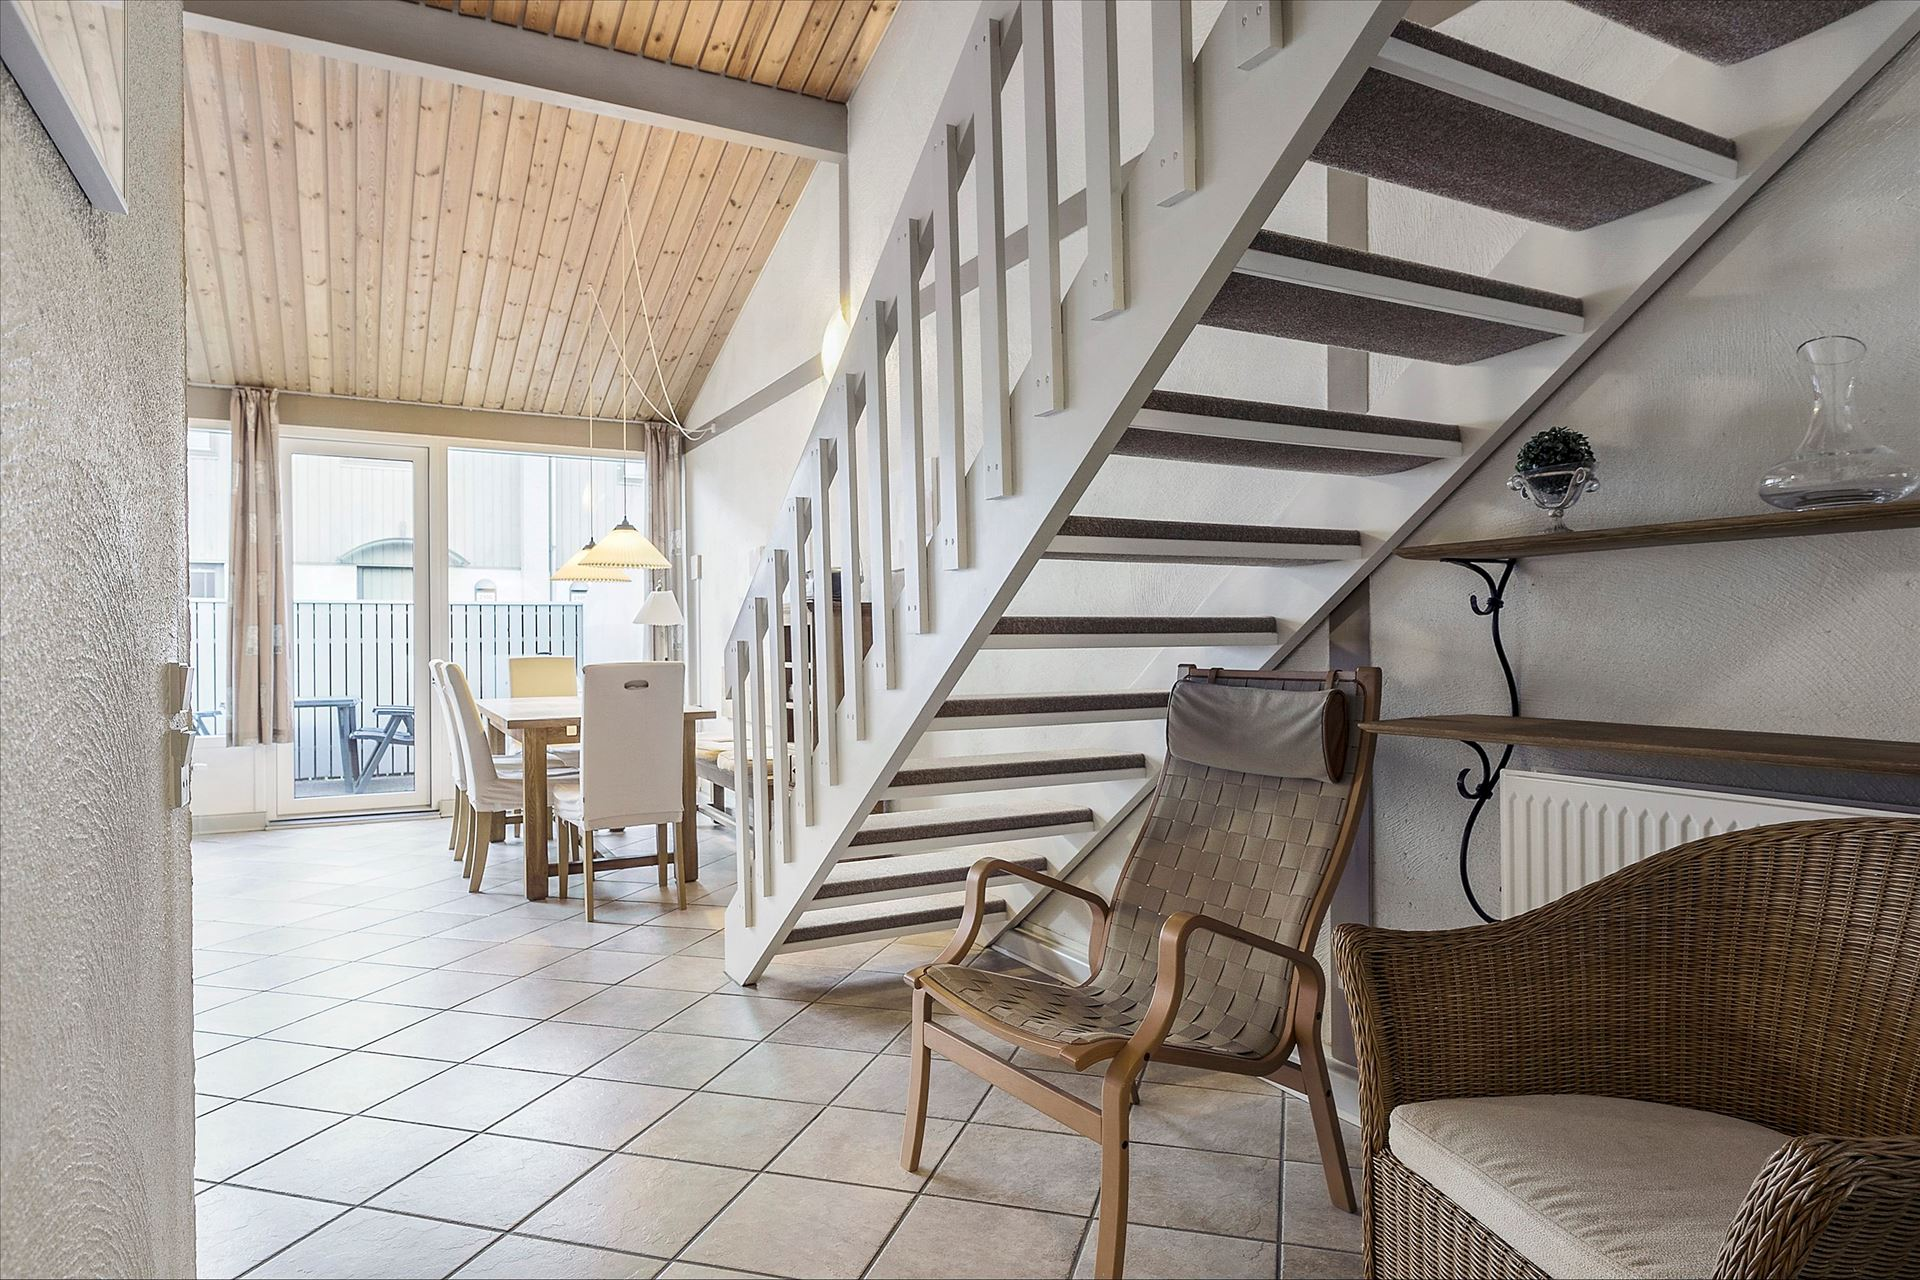
\includegraphics[width=\linewidth]{pictures/random/bexample_entre}
    \caption{Entre}
  \end{subfigure}\hfil % <-- added
  \begin{subfigure}{0.3\textwidth}
    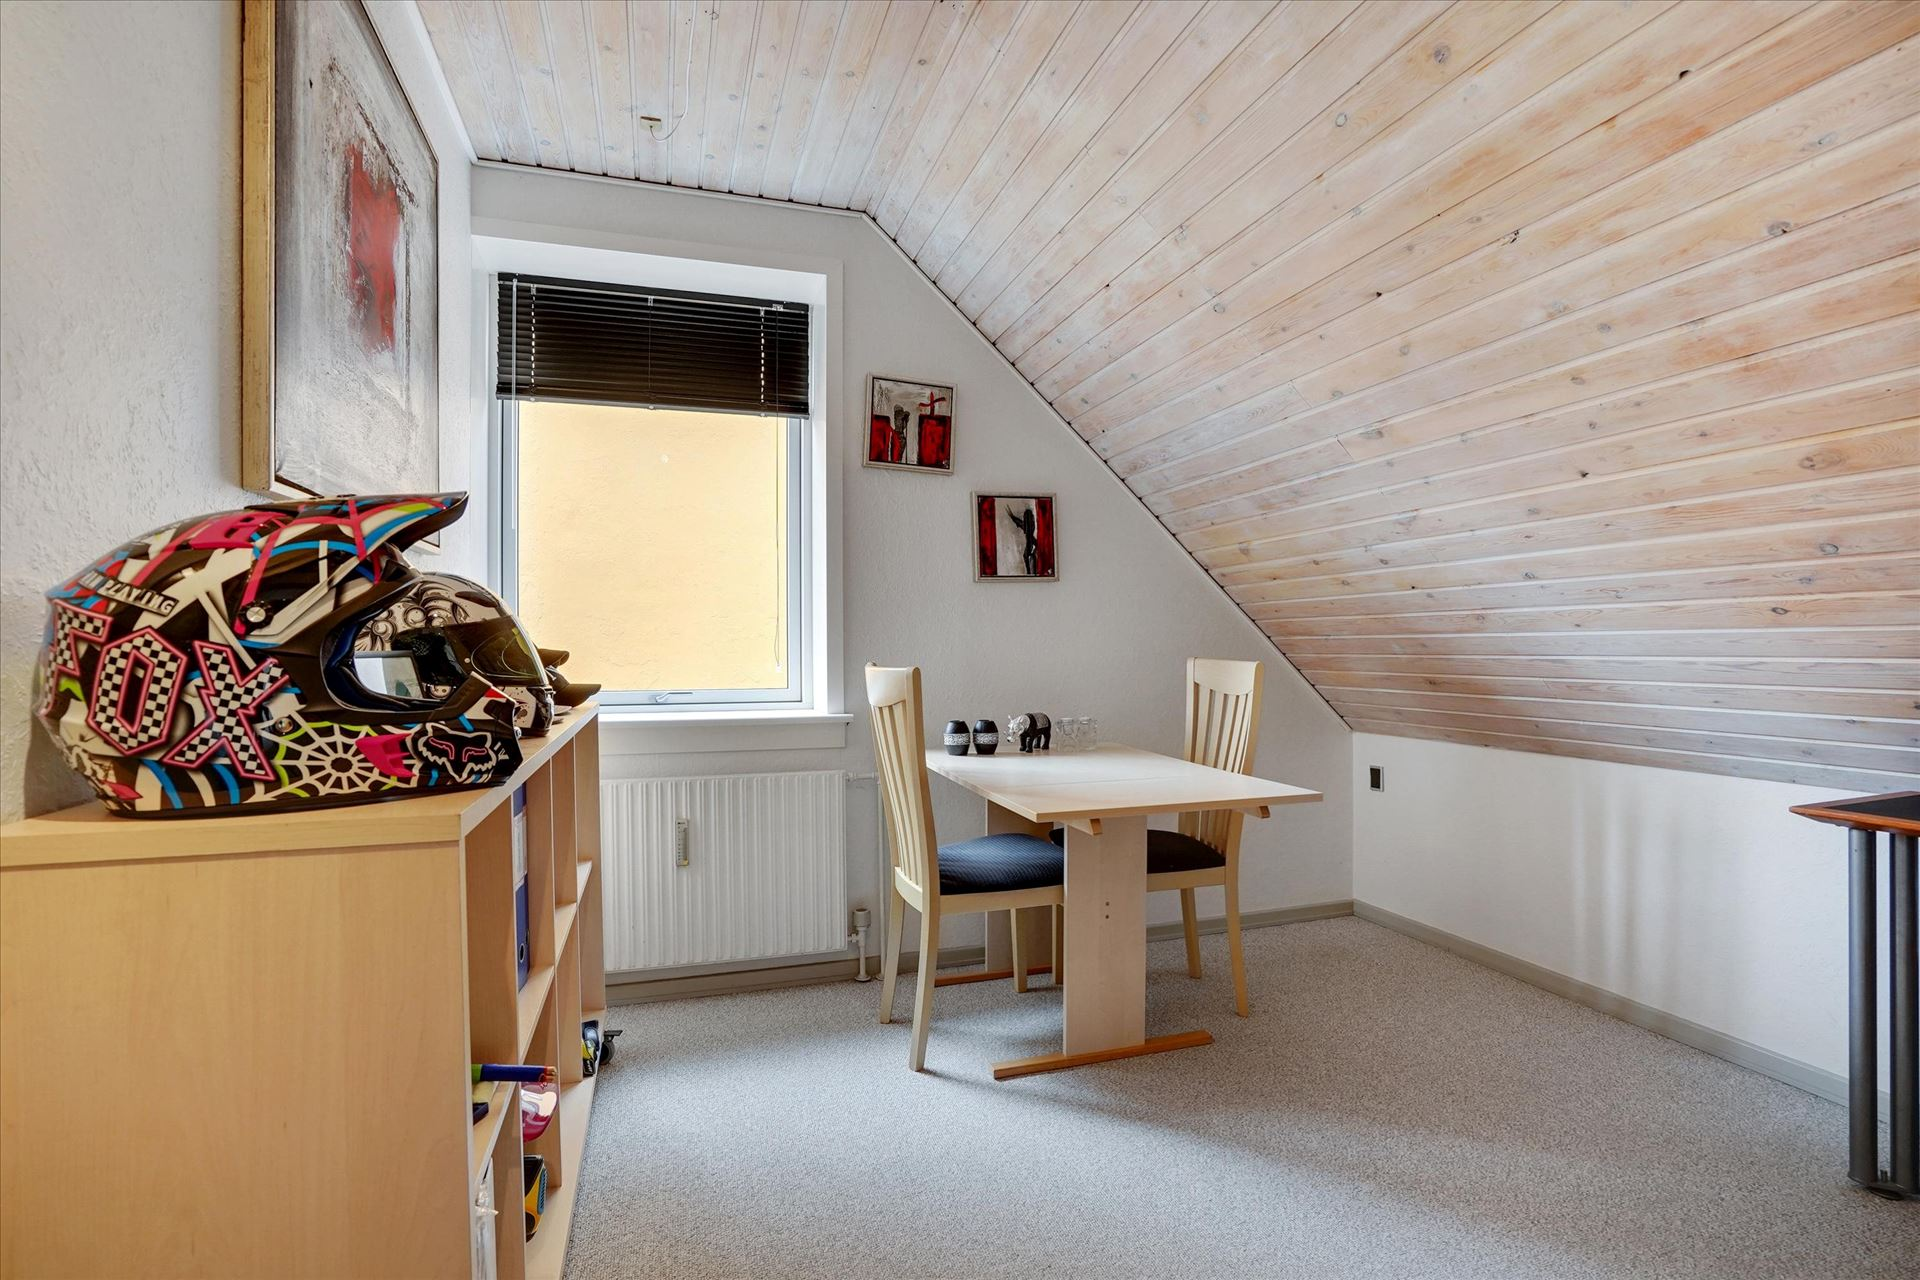
\includegraphics[width=\linewidth]{pictures/random/bexample_diningroom}
    \caption{Dining Room}
  \end{subfigure}
  \caption{Difficult-to-label rooms}
  \label{fig:appb2}
\end{figure}
